\chapter{The Scratch Online Community}
The empirical setting for this work is the Scratch Online Community, a website (Figure~\ref{fig:websitehomepage}), which I conceived and developed over the past three years, for this and other lines research.
The website allows anyone, especially young people between ages 8 and 16, to share their animated stories, interactive art, and video games. Participants use the Scratch programming environment to create or remix projects by putting together images, music and sounds with programming command blocks \citep{resnick_scratch:_2009}.
Projects range from interactive greeting cards, physics simulations, animations of popular songs to homemade video games, just to name a few.  

\begin{figure}
\centering
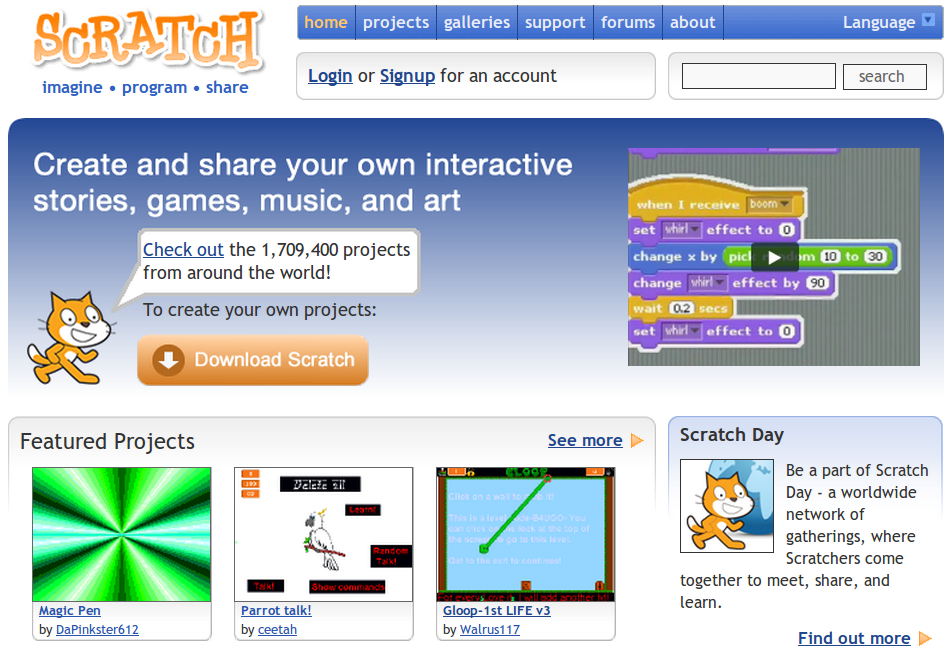
\includegraphics[width=3.25in]{figures/websitehomepage.png}
\caption{The home page of the Scratch website}
\label{fig:homepage}
\end{figure}

\section{Motivations}

I elaborate on the motivations for creating this social space driven by a desire to provide creators with access to a repository of inspirational creations and to a network of peers that can be both audience and co-creators.

% TODO: samba school, minsky literature, consumption to production, audience: peers, collaborators,  repository.

\section{Socio-technical infrastructure}
I provide an in-depth description of the technical and social infrastructure behind the Scratch website and its evolution over the course of three years.  

% TODO: diagram of the system, usage stats, moderation model, user experience, social features
